\PassOptionsToPackage{dvipsnames,svgnames,x11names}{xcolor}
\documentclass[tikz,border=8pt]{standalone}
\usetikzlibrary{arrows.meta,positioning,calc,shapes,shadows,decorations.pathmorphing,shapes.geometric,backgrounds,decorations.markings,decorations.pathreplacing,decorations.text,fit,shapes.misc,shapes.arrows,matrix,bending,3d,chains,intersections,shapes.symbols,svg.path,shapes.multipart,snakes,shapes.callouts,angles,quotes}
\providecolor{gold}{RGB}{212,175,55}
\providecolor{silver}{RGB}{192,192,192}
\providecolor{bronze}{RGB}{205,127,50}
\providecolor{darkblue}{RGB}{0,0,139}
\providecolor{lightblue}{RGB}{173,216,230}
\providecolor{darkgreen}{RGB}{0,100,0}
\providecolor{lightgreen}{RGB}{144,238,144}
\providecolor{darkred}{RGB}{139,0,0}
\providecolor{navy}{RGB}{0,0,128}
\providecolor{skyblue}{RGB}{135,206,235}
\providecolor{beige}{RGB}{245,245,220}
\providecolor{cream}{RGB}{255,253,208}
\usepackage{amsmath}
\usepackage{amssymb}
\usepackage{fontawesome5}
\usetikzlibrary{fadings,shadows.blur,patterns,patterns.meta}

\providecolor{gold}{RGB}{212,175,55}
\providecolor{silver}{RGB}{192,192,192}
\providecolor{bronze}{RGB}{205,127,50}
\providecolor{darkblue}{RGB}{0,0,139}
\providecolor{lightblue}{RGB}{173,216,230}
\providecolor{darkgreen}{RGB}{0,100,0}
\providecolor{lightgreen}{RGB}{144,238,144}
\providecolor{darkred}{RGB}{139,0,0}
\providecolor{navy}{RGB}{0,0,128}
\providecolor{skyblue}{RGB}{135,206,235}
\providecolor{beige}{RGB}{245,245,220}
\providecolor{cream}{RGB}{255,253,208}
\usepackage{amsmath}
\usepackage{amssymb}
\usepackage{fontawesome5}


\usepackage{xcolor}

% --- COLOR PALETTE DEFINITIONS ---
\definecolor{stepcolor}{RGB}{30, 41, 59}        % Slate 800 (Deep technical slate)
\definecolor{stepborder}{RGB}{71, 85, 105}      % Slate 600
\definecolor{accent}{RGB}{14, 165, 233}         % Sky Cyan 500
\definecolor{accentdark}{RGB}{2, 132, 199}      % Sky Cyan 600
\definecolor{accentbg}{RGB}{240, 249, 255}      % Sky 50
\definecolor{warn}{RGB}{234, 88, 12}            % Deep Orange/Amber
\definecolor{warndark}{RGB}{194, 65, 12}        % Orange 700
\definecolor{warnbg}{RGB}{255, 247, 237}        % Orange 50
\definecolor{success}{RGB}{16, 185, 129}        % Emerald 500
\definecolor{successdark}{RGB}{5, 150, 105}     % Emerald 600
\definecolor{successbg}{RGB}{236, 253, 245}     % Emerald 50
\definecolor{codecolor}{RGB}{190, 24, 93}       % Ruby / Magenta for inline syntax
\definecolor{cardbgtop}{RGB}{255, 255, 255}
\definecolor{cardbgbot}{RGB}{248, 250, 252}
\definecolor{marginboxbg}{RGB}{250, 250, 250}
\definecolor{marginborder}{RGB}{203, 213, 225}

\begin{document}
\begin{tikzpicture}[
    font=\sffamily,
    % --- REFINED ARCHITECTURAL STYLES ---
    realistic_node/.style={
        draw=stepborder,
        line width=1.2pt,
        top color=cardbgtop,
        bottom color=cardbgbot,
        rounded corners=8pt,
        inner sep=10pt,
        align=center,
        font=\sffamily,
        blur shadow={shadow blur steps=6, shadow xshift=0pt, shadow yshift=-3pt, shadow opacity=22}
    },
    sniff_node/.style={
        draw=accentdark,
        line width=1.4pt,
        top color=white,
        bottom color=accentbg,
        rounded corners=8pt,
        inner sep=10pt,
        align=center,
        font=\sffamily,
        blur shadow={shadow blur steps=6, shadow xshift=0pt, shadow yshift=-3pt, shadow opacity=25}
    },
    sandbox_node/.style={
        draw=warndark,
        line width=1.4pt,
        top color=white,
        bottom color=warnbg,
        rounded corners=8pt,
        inner sep=10pt,
        align=center,
        font=\sffamily,
        blur shadow={shadow blur steps=6, shadow xshift=0pt, shadow yshift=-3pt, shadow opacity=25}
    },
    handshake_node/.style={
        draw=successdark,
        line width=1.5pt,
        top color=white,
        bottom color=successbg,
        rounded corners=10pt,
        inner sep=12pt,
        align=center,
        font=\sffamily,
        blur shadow={shadow blur steps=8, shadow xshift=0pt, shadow yshift=-4pt, shadow opacity=28}
    },
    resolution_node/.style={
        draw=successdark,
        line width=2pt,
        top color=successbg!40!white,
        bottom color=successbg,
        rounded corners=10pt,
        inner sep=12pt,
        align=center,
        font=\sffamily,
        blur shadow={shadow blur steps=10, shadow xshift=0pt, shadow yshift=-4pt, shadow opacity=32}
    },
    sandbox_boundary/.style={
        draw=warn,
        line width=2pt,
        dashed,
        fill=warn!5,
        rounded corners=15pt
    },
    flow_arrow/.style={
        -Latex=3mm,
        line width=2pt,
        color=stepcolor,
        rounded corners=12pt
    },
    margin_card/.style={
        draw=marginborder,
        line width=1.1pt,
        top color=white,
        bottom color=marginboxbg,
        rounded corners=8pt,
        inner sep=10pt,
        align=left,
        font=\sffamily,
        blur shadow={shadow blur steps=5, shadow xshift=0pt, shadow yshift=-2pt, shadow opacity=16}
    },
    micro_chip/.style={
        draw=stepborder!40,
        fill=white,
        rounded corners=3pt,
        inner sep=3pt,
        font=\scriptsize\ttfamily
    }
]

% ==========================================
% 1. CANVAS BOUNDS
% ==========================================
\fill[white] (-22, -35) rectangle (22,3.4756);

% ==========================================
% 2. TITLE & SUBTITLE
% ==========================================
\node[font=\sffamily\Huge\bfseries, text=stepcolor] at (0,1.9756) {Browser Engine Pipeline: Isolating the Context};
\node[font=\Large\color{gray!80!black}] at (0,0.4756) {The step-by-step rendering timeline constructing the self-contained layout engine};

% ==========================================
% 3. MAIN PRE-SANDBOX PIPELINE
% ==========================================

% --- Step 1: HTML DOM Parser ---
\node[realistic_node, text width=6.5cm] (step1) at (0, -1.5) {
    {\bfseries\color{stepcolor}\faCode \ 1. HTML DOM Parser}\\[3pt]
    encounters \color{codecolor}\texttt{<img>}\color{stepcolor}\ tag\\[5pt]
    \begin{tikzpicture}[baseline=(root.base), scale=0.75, every node/.style={transform shape}]
        \node[micro_chip, fill=stepcolor!5] (root) at (0,0) {HTML};
        \node[micro_chip, fill=stepcolor!5] (body) at (2,0) {BODY};
        \node[micro_chip, fill=accent!15, draw=accent] (img) at (4.5,0) {\textbf{<img\dots>}};
        \draw[line width=0.8pt, stepcolor!50, ->] (root) -- (body);
        \draw[line width=0.8pt, stepcolor!50, ->] (body) -- (img);
    \end{tikzpicture}
};

% --- Step 2: Network Layer ---
\node[realistic_node, text width=6.5cm] (step2) at (0, -6.0) {
    {\bfseries\color{stepcolor}\faServer \ 2. Network Layer}\\[3pt]
    Executes HTTP GET\\[5pt]
    \begin{tikzpicture}[baseline=(p1.base), scale=0.75, every node/.style={transform shape}]
        \node[micro_chip, fill=accentbg, draw=accent] (p1) at (0,0) {Client};
        \node[micro_chip, fill=stepcolor!5] (p2) at (5,0) {Remote Asset};
        \draw[line width=0.9pt, accentdark, -Latex] (0.8, 0.3) -- node[above=4pt, font=\scriptsize\bfseries]{GET /vector.svg} (4.2, 0.3);
        \draw[line width=0.9pt, successdark, -Latex] (4.2, -0.3) -- node[below=4pt, font=\scriptsize\bfseries]{200 OK (Stream)} (0.8, -0.3);
    \end{tikzpicture}
};

% --- Step 3: Content Sniffing ---
\node[sniff_node, text width=6.5cm] (step3) at (0, -10.5) {
    {\bfseries\color{accentdark}\faSearch \ 3. Content Sniffing}\\[3pt]
    Identifies \color{codecolor}\texttt{image/svg+xml}\color{stepcolor}\\[5pt]
    \begin{tikzpicture}[scale=0.8, every node/.style={transform shape}]
        \node[micro_chip, fill=accent!20, draw=accentdark] at (0,0) {\faFileCode \ MIME: \texttt{image/svg+xml}};
    \end{tikzpicture}
};

% ==========================================
% 4. THE ISOLATED SVG CONTEXT (THE SANDBOX)
% ==========================================

% Sandbox Enclave Outer Boundary (Drawn FIRST so Header and Badge mask it)
\draw[sandbox_boundary] (-11.5, -14.0) rectangle (11.5, -32.5);

% Sandbox Header (Drawn SECOND with fill=white and inner sep=10pt to mask boundary)
\node[font=\LARGE\bfseries, text=warndark, fill=white, draw=warn!60, line width=1.2pt, rounded corners=8pt, inner sep=10pt, blur shadow={shadow blur steps=4, shadow opacity=20}] (sandbox_header) at (0, -14.0) {
    \faLock \ Isolated SVG Context (The Sandbox)
};

% --- Step 4a: SVG DOM Construction ---
\node[sandbox_node, text width=6cm] (step4a) at (-5.5, -18.0) {
    {\bfseries\color{warndark}\faSitemap \ 4a. Parse XML Array}\\[3pt]
    Construct SVG DOM\\[6pt]
    \begin{tikzpicture}[scale=0.72, every node/.style={transform shape}]
        \node[micro_chip, fill=warnbg, draw=warndark] (svg) at (0, 0.4) {<svg>};
        \node[micro_chip, fill=warn!10] (g) at (-1.6, -0.7) {<g>};
        \node[micro_chip, fill=warn!10] (p) at (1.6, -0.7) {<path>};
        \draw[line width=0.8pt, warndark!60] (svg.south) -- (g.north);
        \draw[line width=0.8pt, warndark!60] (svg.south) -- (p.north);
    \end{tikzpicture}
};

% --- Step 4b: SVG CSSOM Construction ---
\node[sandbox_node, text width=6cm] (step4b) at (5.5, -18.0) {
    {\bfseries\color{warndark}\faCss3* \ 4b. Parse Embedded CSS}\\[3pt]
    Construct SVG CSSOM\\[6pt]
    \begin{tikzpicture}[scale=0.72, every node/.style={transform shape}]
        \node[micro_chip, fill=warnbg, draw=warndark] (style) at (0, 0.4) {<style>};
        \node[micro_chip, fill=warn!10] (r1) at (-1.6, -0.7) {.cls-1 \{fill\dots\}};
        \node[micro_chip, fill=warn!10] (r2) at (1.6, -0.7) {@media (\dots)};
        \draw[line width=0.8pt, warndark!60] (style.south) -- (r1.north);
        \draw[line width=0.8pt, warndark!60] (style.south) -- (r2.north);
    \end{tikzpicture}
};

% --- Step 5: The Viewport Delegation Handshake ---
\node[handshake_node, text width=10cm] (step5) at (0, -24.5) {
    {\bfseries\color{successdark}\faVectorSquare \ 5. The Viewport Delegation Handshake}\\[4pt]
    Host HTML DOM calculates \color{codecolor}\texttt{<img>}\color{stepcolor}\ box size\\[2pt]
    Injects \textbf{\color{successdark}$(Width, Height)$} into Sandbox Engine\\[6pt]
    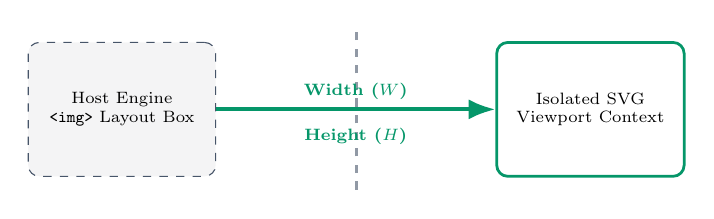
\begin{tikzpicture}[scale=0.85, every node/.style={transform shape}]
        % Host DOM Representation (External Box)
        \node[draw=stepborder, dashed, fill=stepcolor!5, minimum width=2.8cm, minimum height=2cm, align=center, font=\scriptsize, rounded corners=4pt] (host) at (-3.5, 0) {Host Engine \\ \texttt{<img>} Layout Box};
        % SVG Sandbox Viewport (Internal Context)
        \node[draw=successdark, fill=white, line width=1pt, minimum width=2.8cm, minimum height=2cm, align=center, font=\scriptsize, rounded corners=4pt] (svg) at (3.5, 0) {Isolated SVG \\ Viewport Context};
        % Strict Isolation Boundary Line
        \draw[draw=stepborder!60, dashed, line width=1pt] (0, -1.2) -- (0, 1.2);
        % Injected Delegation Arrow across boundary
        \draw[-Latex, successdark, line width=1.5pt] (host.east) -- node[above, font=\scriptsize\bfseries]{Width ($W$)} node[below=4pt, font=\scriptsize\bfseries]{Height ($H$)} (svg.west);
    \end{tikzpicture}
};

% --- Step 6: Media Query Layout Resolution ---
\node[resolution_node, text width=10cm] (step6) at (0, -30.0) {
    {\bfseries\color{successdark}\faSlidersH \ 6. Media Query Layout Resolution}\\[4pt]
    SVG CSSOM resolves \color{codecolor}\texttt{@media}\color{stepcolor}\ variables\\[2pt]
    using the delegated bounds. Paint occurs. \ \color{successdark}\faPaintBrush\\[6pt]
    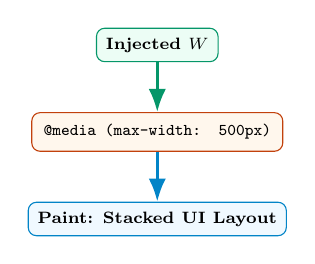
\begin{tikzpicture}[scale=0.85, every node/.style={transform shape}]
        \node[draw=successdark, fill=successbg, font=\scriptsize\bfseries, rounded corners=3pt, inner sep=4pt] (w) at (0, 1.3) {Injected $W$};
        \node[draw=warndark, fill=warnbg, font=\scriptsize\ttfamily, rounded corners=3pt, inner sep=5pt] (mq) at (0,0) {@media (max-width: 500px)};
        \node[draw=accentdark, fill=accentbg, font=\scriptsize\bfseries, rounded corners=3pt, inner sep=4pt] (paint) at (0, -1.3) {Paint: Stacked UI Layout};
        \draw[-Latex, successdark, line width=1.2pt] (w.south) -- (mq.north);
        \draw[-Latex, accentdark, line width=1.2pt] (mq.south) -- (paint.north);
    \end{tikzpicture}
};

% Bottom Verification Badge (Drawn with fill=white and inner sep=10pt to mask boundary)
\node[font=\bfseries, text=successdark, fill=white, draw=success, line width=1.2pt, rounded corners=6pt, inner sep=10pt, blur shadow={shadow blur steps=4, shadow opacity=18}] at (-0.0399,-33.3771) {
    \faCheckCircle \ Mathematical substitution complete
};

% ==========================================
% 5. FLUID PIPELINE ROUTING & ARROWS
% ==========================================

% Step 1 to Step 2
\draw[flow_arrow] (step1.south) -- (step2.north);

% Step 2 to Step 3
\draw[flow_arrow] (step2.south) -- (step3.north);

% Step 3 to Sandbox Gateway (crosses boundary into isolation via sandbox_header)
\draw[flow_arrow] (step3.south) -- (sandbox_header.north);
\draw[flow_arrow] (sandbox_header.south) -- (0, -15.5);

% Split inside sandbox to Steps 4a & 4b
\draw[line width=2pt, color=stepcolor] (-5.5, -15.5) -- (5.5, -15.5);
\draw[flow_arrow] (-5.5, -15.5) -- (step4a.north);
\draw[flow_arrow] (5.5, -15.5) -- (step4b.north);

% Merge Steps 4a & 4b into Step 5
\draw[flow_arrow] (step4a.south) -- ++(0,-1.5) -| (step5.north);
\draw[flow_arrow] (step4b.south) -- ++(0,-1.5) -| (step5.north);

% Step 5 to Step 6
\draw[flow_arrow] (step5.south) -- (step6.north);

% ==========================================
% 6. MARGIN EXPLANATORY NOTES
% ==========================================

% --- Left Margin Card: Security & Layout Boundary ---
\node[margin_card, text width=5.5cm] (left_card) at (-16, -18.0) {
    {\bfseries\color{warndark}\faIcon{shield-alt} \ Security \& Layout Boundary}\\[5pt]
    The browser restricts the SVG from:\\[3pt]
    \textbullet \ Accessing host JS\\
    \textbullet \ Accessing host CSS stylesheets\\
    \textbullet \ Overflowing its bounding box
};
\draw[-Stealth, warndark, dashed, line width=1.5pt] (left_card.east) -- (-11.5, -18.0);

% --- Right Margin Card: The Delegation Handshake ---
\node[margin_card, text width=6.5cm] (right_card) at (16, -24.5) {
    {\bfseries\color{accentdark}\faIcon{exchange-alt} \ The Delegation Handshake}\\[5pt]
    The primary engine instructs:\\[3pt]
    \textit{"I computed your box to be 300px wide. Execute your internal CSS assuming your 'window' is precisely 300px."}
};
\draw[-Stealth, successdark, dashed, line width=1.5pt] (right_card.west) -- (step5.east);

\end{tikzpicture}
\end{document}
